As in the ECAL energy reconstruction, the ratio-based timing method estimates the time of a reconstructed hit (rechit) from the ten consecutively sampled pulse amplitudes recorded at 25\,ns intervals.
For an isolated signal with the expected pulse shape, the ratio of any two consecutive amplitude samples uniquely determines the relative timing of the pulse with respect to the LHC clock.
Figure~\ref{tec_pulseratio} shows the ratio
\[
R = \frac{A(T)}{A(T+25\,\mathrm{ns})}
\]
as a function of the time difference $T - T_{\mathrm{max}}$, where $T_{\mathrm{max}}$ denotes the time at which the pulse reaches its maximum amplitude.

The first three sampled amplitudes, $A(1)$, $A(2)$, and $A(3)$, are typically used to determine the pedestal value corresponding to zero signal and are therefore excluded from the timing reconstruction.
Ratios formed from $R\!\left(A(4)/A(5)\right)$ through $R\!\left(A(7)/A(8)\right)$ are used to estimate the pulse time.
Ratios involving samples on the falling tail of the pulse provide little sensitivity to the pulse timing and are not utilized.
The rechit time is determined from a weighted average of three consecutive ratio-based timing estimates derived from these sample pairs.

\begin{figure}[htbp]
\begin{center}
\resizebox{0.7\linewidth}{!}{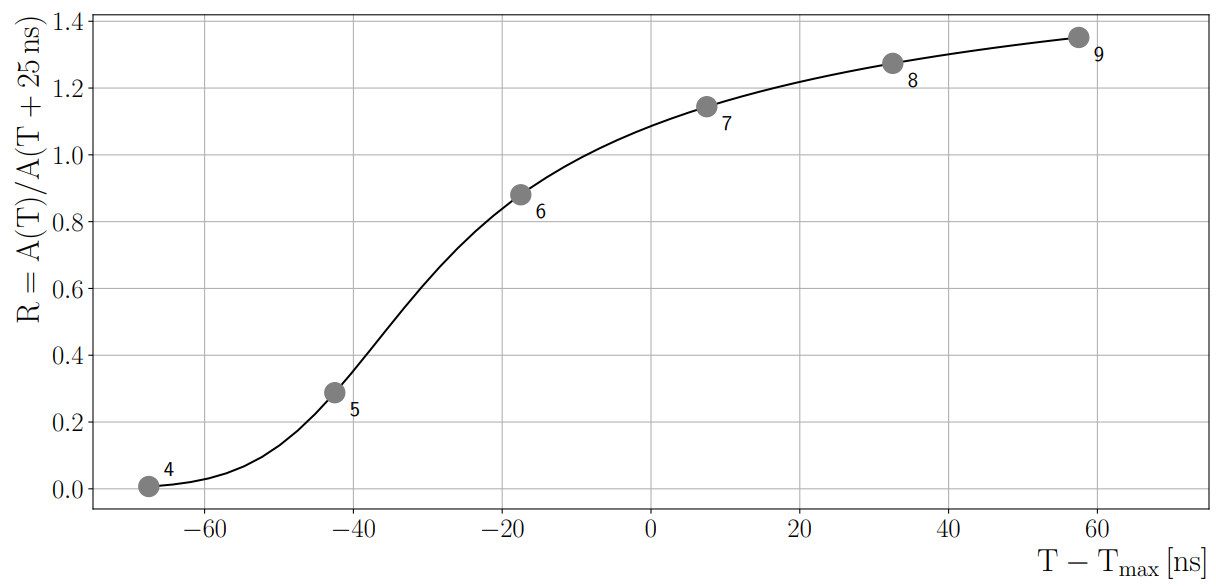
\includegraphics{fig/sec_reco/ratio_tvR_mod.png}}
\caption{Ratio $R$ of two consecutive pulse amplitudes, $A(T)$ and $A(T+25\,\mathrm{ns})$, as a function of the time difference $T - T_{\mathrm{max}}$.
The first three samples, $A(1)$--$A(3)$, which are used for pedestal determination, are excluded.
The rechit time is obtained from a weighted average of the timing estimates derived from the ratios $R\!\left(A(4)/A(5)\right)$ through $R\!\left(A(7)/A(8)\right)$.}
\label{tec_pulseratio}
\end{center}
\end{figure}

Channel-dependent delays in the clock distribution system introduce offsets between the reconstructed pulse time and the true particle arrival time.
These offsets vary from crystal to crystal and are corrected using calibration constants derived from prompt relativistic particles, such that the mean reconstructed time for each channel is centered at zero~\cite{CMS-PAS-EXO-19-005}.

The time of arrival of a reconstructed particle at the ECAL, $t_{\mathrm{ECAL}}$, is computed as a weighted average of the rechit times from the individual crystals comprising the associated ECAL cluster,
\begin{equation}
t_{\mathrm{ECAL}} =
\frac{\sum_{i} t^{i}_{\mathrm{ECAL}} / \sigma^{2}_{i}}
     {\sum_{i} 1 / \sigma^{2}_{i}} \, ,
\label{ratio_eqt}
\end{equation}
where $t^{i}_{\mathrm{ECAL}}$ is the reconstructed time of the rechit in crystal $i$ and $\sigma_{i}$ is the estimated time resolution for that crystal.
The resolution weights $\sigma_{i}$ are derived from the intrinsic timing performance of the ECAL crystal and readout system~\cite{Collaboration_2010}.

The ratio-based timing method assumes that the sampled signal pulse is well isolated in time.
In the higher pileup environments of Run~II and Run~III, this assumption is no longer valid.
As discussed previously, the observed pulse shape in an ECAL channel is generally a superposition of an in-time pulse and multiple non-negligible out-of-time contributions arising from pileup and out-of-time pileup (OOT-PU).
In such cases, the sampled pulse shape deviates significantly from the nominal pulse template.
When this occurs, the ratio of two consecutive samples no longer provides a unique mapping to the pulse time, resulting in degraded timing resolution and increased sensitivity to pileup-induced biases.
